\documentclass[landscape]{beamer}
\usepackage{bm}
\usepackage{harpoon}
\usepackage{fontspec}
\usepackage{listings}
\usepackage{setspace}
\usepackage{color}
\usepackage{cmap}
\usepackage{cite}
\usepackage{tikz}
\usepackage{esvect}
\usepackage{float}
\usepackage{xeCJK}
\usepackage{amsthm}
\usepackage{amsmath}
\usepackage{amssymb}
\usepackage{setspace}
\usepackage{enumerate}
\usepackage{multicol}
\usepackage{indentfirst}
\usepackage{subfigure}
\usepackage{hyperref}
%\setlength{\parindent}{0em}
%\setlength{\mathindent}{0pt}
\usetheme{Warsaw}
%\usecolortheme{beaver}

\begin{document}
	\title{\textbf{Balanced Programming}}
	\author{Group Static}
	\institute{Shanghai Jiao Tong University}
	\maketitle
	\section*{Introduction}
	\begin{frame}
		\frametitle{Introduction}
		\begin{itemize}
			\item Very useful idea when confronting the following cases:\pause
			\begin{enumerate}
				\item There are two algorithms, both of which have different features, such as one has
				lower complexity in query and the other has lower complexity in modification.\pause
				\item The whole problem can be divided into several problems called ``big problems'' and these problems can be also
				divided into several smaller but common problems called ``small problems''.\pause
			\end{enumerate}
			\item The main idea is these algorithms learning from each other.
		\end{itemize}
	\end{frame}
	\section{Meet in the middle}
	% xzj Part
	\begin{frame}[c]\frametitle{Meet in the middle}
		\begin{columns}
			\column{4cm}
			\begin{itemize}
				\item<1-> Given an undirected graph whose nodes' degree is 5 and find a path from $S$ to $T$.
				\item<2-> dist(S, T) = L
				\item<3-> $O(4^L)$
				\item<4-> Meet in the middle
				\item<4-> $O(4^{L/2})$
			\end{itemize}
			\column{6cm}
			\only{\centering{{\includegraphics[width=6cm]{img/pic0.png}<1-2>}}}
			\only{\centering{{\includegraphics[width=6cm]{img/pic1.png}<3>}}}
			\only{\centering{{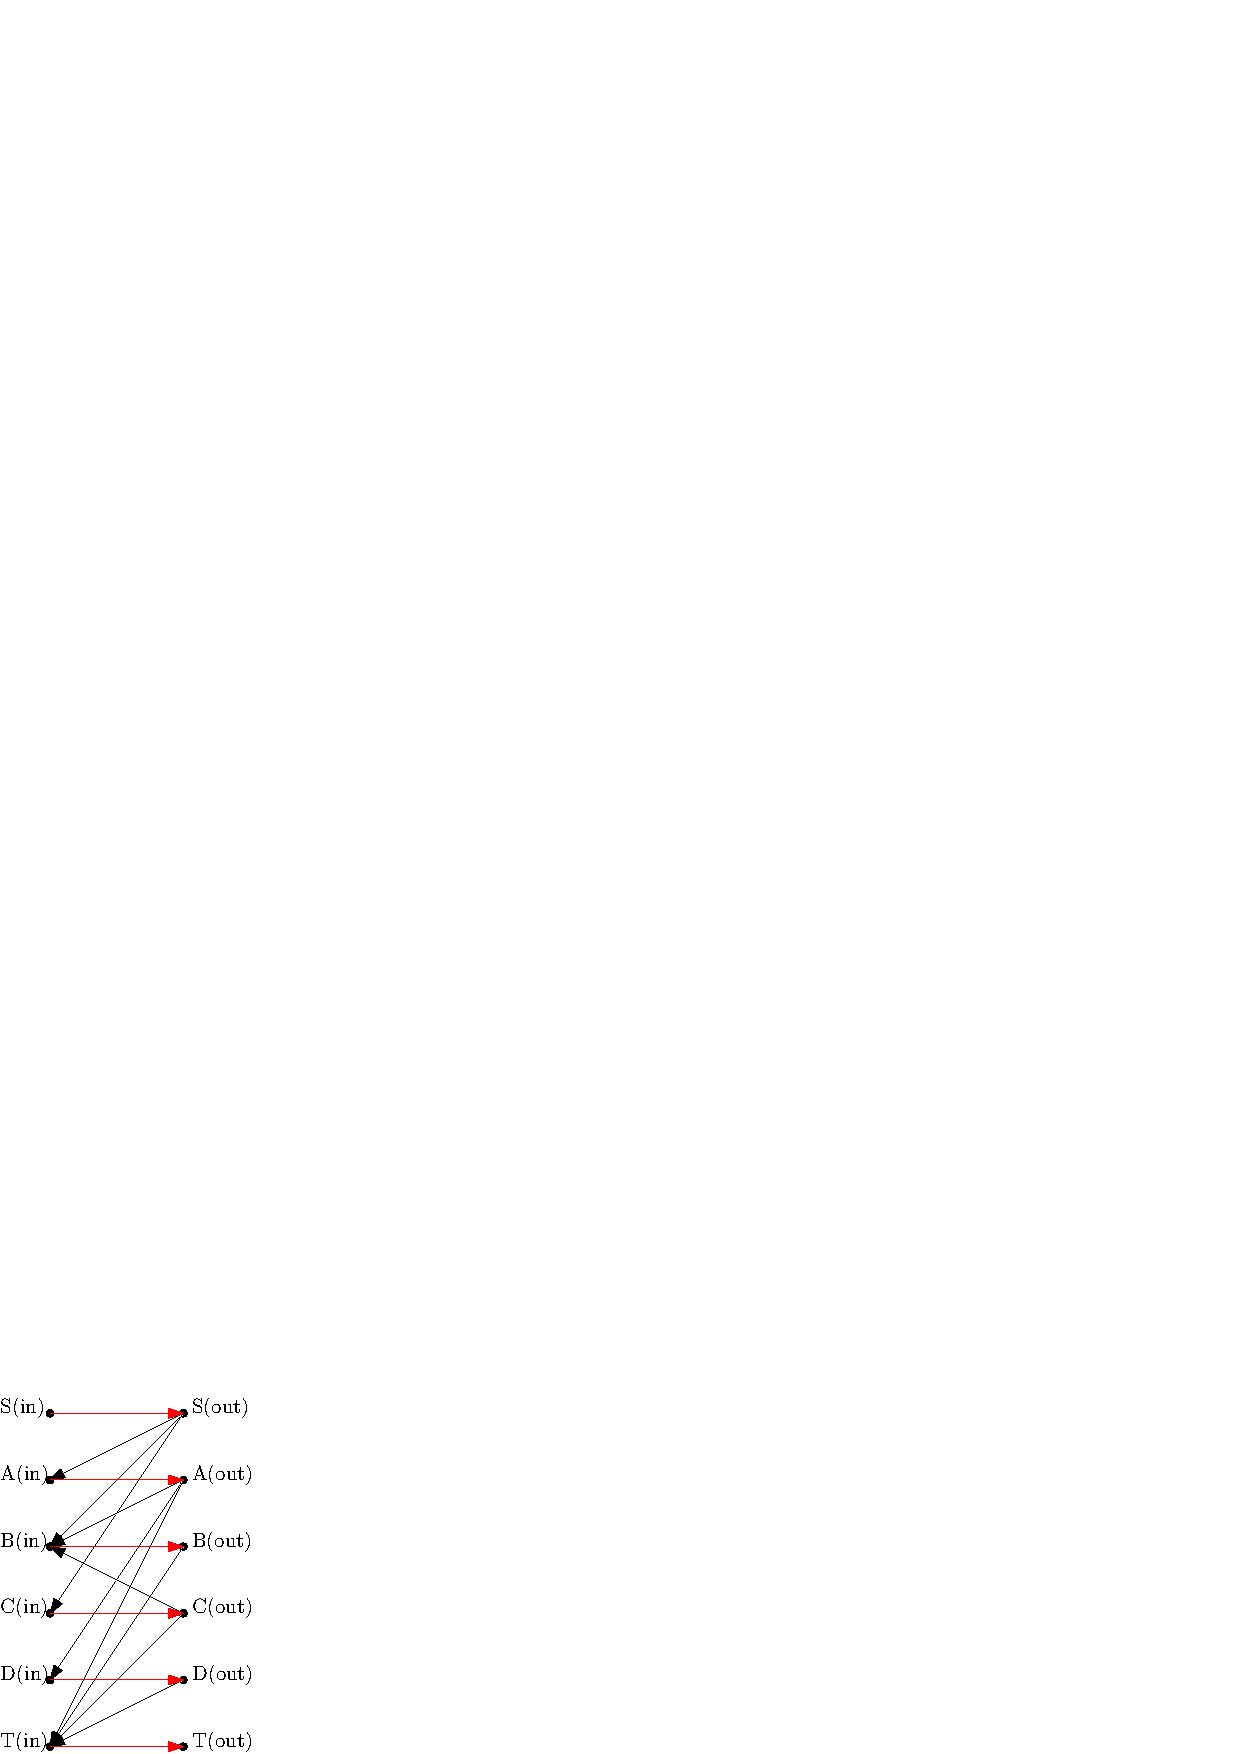
\includegraphics[width=7cm]{img/pic2.png}<4>}}}
		\end{columns}
	\end{frame}
	\begin{frame}[c]\frametitle{Some other applications}
		\begin{columns}
			\column{4cm}
			\beamerdefaultoverlayspecification{<+->}
			\begin{itemize}
				\item Mo's algorithm
				\item Bolcked list
				\item Dinic(capacity is 1)
				\item ......
			\end{itemize}
			\column{7cm}
			\only{\centering{{\includegraphics[width=7cm]{img/bl.png}<2>}}}
		\end{columns}
	\end{frame}
	\section{Thanks}
	\begin{frame}
		\frametitle{Thanks}
		Thanks for listening.\\
		Questions are welcomed.
	\end{frame}
\end{document}
